
% Default to the notebook output style

    


% Inherit from the specified cell style.




    
\documentclass[11pt]{article}

    
    
    \usepackage[T1]{fontenc}
    % Nicer default font (+ math font) than Computer Modern for most use cases
    \usepackage{mathpazo}

    % Basic figure setup, for now with no caption control since it's done
    % automatically by Pandoc (which extracts ![](path) syntax from Markdown).
    \usepackage{graphicx}
    % We will generate all images so they have a width \maxwidth. This means
    % that they will get their normal width if they fit onto the page, but
    % are scaled down if they would overflow the margins.
    \makeatletter
    \def\maxwidth{\ifdim\Gin@nat@width>\linewidth\linewidth
    \else\Gin@nat@width\fi}
    \makeatother
    \let\Oldincludegraphics\includegraphics
    % Set max figure width to be 80% of text width, for now hardcoded.
    \renewcommand{\includegraphics}[1]{\Oldincludegraphics[width=.8\maxwidth]{#1}}
    % Ensure that by default, figures have no caption (until we provide a
    % proper Figure object with a Caption API and a way to capture that
    % in the conversion process - todo).
    \usepackage{caption}
    \DeclareCaptionLabelFormat{nolabel}{}
    \captionsetup{labelformat=nolabel}

    \usepackage{adjustbox} % Used to constrain images to a maximum size 
    \usepackage{xcolor} % Allow colors to be defined
    \usepackage{enumerate} % Needed for markdown enumerations to work
    \usepackage{geometry} % Used to adjust the document margins
    \usepackage{amsmath} % Equations
    \usepackage{amssymb} % Equations
    \usepackage{textcomp} % defines textquotesingle
    % Hack from http://tex.stackexchange.com/a/47451/13684:
    \AtBeginDocument{%
        \def\PYZsq{\textquotesingle}% Upright quotes in Pygmentized code
    }
    \usepackage{upquote} % Upright quotes for verbatim code
    \usepackage{eurosym} % defines \euro
    \usepackage[mathletters]{ucs} % Extended unicode (utf-8) support
    \usepackage[utf8x]{inputenc} % Allow utf-8 characters in the tex document
    \usepackage{fancyvrb} % verbatim replacement that allows latex
    \usepackage{grffile} % extends the file name processing of package graphics 
                         % to support a larger range 
    % The hyperref package gives us a pdf with properly built
    % internal navigation ('pdf bookmarks' for the table of contents,
    % internal cross-reference links, web links for URLs, etc.)
    \usepackage{hyperref}
    \usepackage{longtable} % longtable support required by pandoc >1.10
    \usepackage{booktabs}  % table support for pandoc > 1.12.2
    \usepackage[inline]{enumitem} % IRkernel/repr support (it uses the enumerate* environment)
    \usepackage[normalem]{ulem} % ulem is needed to support strikethroughs (\sout)
                                % normalem makes italics be italics, not underlines
    

    
    
    % Colors for the hyperref package
    \definecolor{urlcolor}{rgb}{0,.145,.698}
    \definecolor{linkcolor}{rgb}{.71,0.21,0.01}
    \definecolor{citecolor}{rgb}{.12,.54,.11}

    % ANSI colors
    \definecolor{ansi-black}{HTML}{3E424D}
    \definecolor{ansi-black-intense}{HTML}{282C36}
    \definecolor{ansi-red}{HTML}{E75C58}
    \definecolor{ansi-red-intense}{HTML}{B22B31}
    \definecolor{ansi-green}{HTML}{00A250}
    \definecolor{ansi-green-intense}{HTML}{007427}
    \definecolor{ansi-yellow}{HTML}{DDB62B}
    \definecolor{ansi-yellow-intense}{HTML}{B27D12}
    \definecolor{ansi-blue}{HTML}{208FFB}
    \definecolor{ansi-blue-intense}{HTML}{0065CA}
    \definecolor{ansi-magenta}{HTML}{D160C4}
    \definecolor{ansi-magenta-intense}{HTML}{A03196}
    \definecolor{ansi-cyan}{HTML}{60C6C8}
    \definecolor{ansi-cyan-intense}{HTML}{258F8F}
    \definecolor{ansi-white}{HTML}{C5C1B4}
    \definecolor{ansi-white-intense}{HTML}{A1A6B2}

    % commands and environments needed by pandoc snippets
    % extracted from the output of `pandoc -s`
    \providecommand{\tightlist}{%
      \setlength{\itemsep}{0pt}\setlength{\parskip}{0pt}}
    \DefineVerbatimEnvironment{Highlighting}{Verbatim}{commandchars=\\\{\}}
    % Add ',fontsize=\small' for more characters per line
    \newenvironment{Shaded}{}{}
    \newcommand{\KeywordTok}[1]{\textcolor[rgb]{0.00,0.44,0.13}{\textbf{{#1}}}}
    \newcommand{\DataTypeTok}[1]{\textcolor[rgb]{0.56,0.13,0.00}{{#1}}}
    \newcommand{\DecValTok}[1]{\textcolor[rgb]{0.25,0.63,0.44}{{#1}}}
    \newcommand{\BaseNTok}[1]{\textcolor[rgb]{0.25,0.63,0.44}{{#1}}}
    \newcommand{\FloatTok}[1]{\textcolor[rgb]{0.25,0.63,0.44}{{#1}}}
    \newcommand{\CharTok}[1]{\textcolor[rgb]{0.25,0.44,0.63}{{#1}}}
    \newcommand{\StringTok}[1]{\textcolor[rgb]{0.25,0.44,0.63}{{#1}}}
    \newcommand{\CommentTok}[1]{\textcolor[rgb]{0.38,0.63,0.69}{\textit{{#1}}}}
    \newcommand{\OtherTok}[1]{\textcolor[rgb]{0.00,0.44,0.13}{{#1}}}
    \newcommand{\AlertTok}[1]{\textcolor[rgb]{1.00,0.00,0.00}{\textbf{{#1}}}}
    \newcommand{\FunctionTok}[1]{\textcolor[rgb]{0.02,0.16,0.49}{{#1}}}
    \newcommand{\RegionMarkerTok}[1]{{#1}}
    \newcommand{\ErrorTok}[1]{\textcolor[rgb]{1.00,0.00,0.00}{\textbf{{#1}}}}
    \newcommand{\NormalTok}[1]{{#1}}
    
    % Additional commands for more recent versions of Pandoc
    \newcommand{\ConstantTok}[1]{\textcolor[rgb]{0.53,0.00,0.00}{{#1}}}
    \newcommand{\SpecialCharTok}[1]{\textcolor[rgb]{0.25,0.44,0.63}{{#1}}}
    \newcommand{\VerbatimStringTok}[1]{\textcolor[rgb]{0.25,0.44,0.63}{{#1}}}
    \newcommand{\SpecialStringTok}[1]{\textcolor[rgb]{0.73,0.40,0.53}{{#1}}}
    \newcommand{\ImportTok}[1]{{#1}}
    \newcommand{\DocumentationTok}[1]{\textcolor[rgb]{0.73,0.13,0.13}{\textit{{#1}}}}
    \newcommand{\AnnotationTok}[1]{\textcolor[rgb]{0.38,0.63,0.69}{\textbf{\textit{{#1}}}}}
    \newcommand{\CommentVarTok}[1]{\textcolor[rgb]{0.38,0.63,0.69}{\textbf{\textit{{#1}}}}}
    \newcommand{\VariableTok}[1]{\textcolor[rgb]{0.10,0.09,0.49}{{#1}}}
    \newcommand{\ControlFlowTok}[1]{\textcolor[rgb]{0.00,0.44,0.13}{\textbf{{#1}}}}
    \newcommand{\OperatorTok}[1]{\textcolor[rgb]{0.40,0.40,0.40}{{#1}}}
    \newcommand{\BuiltInTok}[1]{{#1}}
    \newcommand{\ExtensionTok}[1]{{#1}}
    \newcommand{\PreprocessorTok}[1]{\textcolor[rgb]{0.74,0.48,0.00}{{#1}}}
    \newcommand{\AttributeTok}[1]{\textcolor[rgb]{0.49,0.56,0.16}{{#1}}}
    \newcommand{\InformationTok}[1]{\textcolor[rgb]{0.38,0.63,0.69}{\textbf{\textit{{#1}}}}}
    \newcommand{\WarningTok}[1]{\textcolor[rgb]{0.38,0.63,0.69}{\textbf{\textit{{#1}}}}}
    
    
    % Define a nice break command that doesn't care if a line doesn't already
    % exist.
    \def\br{\hspace*{\fill} \\* }
    % Math Jax compatability definitions
    \def\gt{>}
    \def\lt{<}
    % Document parameters
    \title{Central-Limit-Theorem}
    
    
    

    % Pygments definitions
    
\makeatletter
\def\PY@reset{\let\PY@it=\relax \let\PY@bf=\relax%
    \let\PY@ul=\relax \let\PY@tc=\relax%
    \let\PY@bc=\relax \let\PY@ff=\relax}
\def\PY@tok#1{\csname PY@tok@#1\endcsname}
\def\PY@toks#1+{\ifx\relax#1\empty\else%
    \PY@tok{#1}\expandafter\PY@toks\fi}
\def\PY@do#1{\PY@bc{\PY@tc{\PY@ul{%
    \PY@it{\PY@bf{\PY@ff{#1}}}}}}}
\def\PY#1#2{\PY@reset\PY@toks#1+\relax+\PY@do{#2}}

\expandafter\def\csname PY@tok@w\endcsname{\def\PY@tc##1{\textcolor[rgb]{0.73,0.73,0.73}{##1}}}
\expandafter\def\csname PY@tok@c\endcsname{\let\PY@it=\textit\def\PY@tc##1{\textcolor[rgb]{0.25,0.50,0.50}{##1}}}
\expandafter\def\csname PY@tok@cp\endcsname{\def\PY@tc##1{\textcolor[rgb]{0.74,0.48,0.00}{##1}}}
\expandafter\def\csname PY@tok@k\endcsname{\let\PY@bf=\textbf\def\PY@tc##1{\textcolor[rgb]{0.00,0.50,0.00}{##1}}}
\expandafter\def\csname PY@tok@kp\endcsname{\def\PY@tc##1{\textcolor[rgb]{0.00,0.50,0.00}{##1}}}
\expandafter\def\csname PY@tok@kt\endcsname{\def\PY@tc##1{\textcolor[rgb]{0.69,0.00,0.25}{##1}}}
\expandafter\def\csname PY@tok@o\endcsname{\def\PY@tc##1{\textcolor[rgb]{0.40,0.40,0.40}{##1}}}
\expandafter\def\csname PY@tok@ow\endcsname{\let\PY@bf=\textbf\def\PY@tc##1{\textcolor[rgb]{0.67,0.13,1.00}{##1}}}
\expandafter\def\csname PY@tok@nb\endcsname{\def\PY@tc##1{\textcolor[rgb]{0.00,0.50,0.00}{##1}}}
\expandafter\def\csname PY@tok@nf\endcsname{\def\PY@tc##1{\textcolor[rgb]{0.00,0.00,1.00}{##1}}}
\expandafter\def\csname PY@tok@nc\endcsname{\let\PY@bf=\textbf\def\PY@tc##1{\textcolor[rgb]{0.00,0.00,1.00}{##1}}}
\expandafter\def\csname PY@tok@nn\endcsname{\let\PY@bf=\textbf\def\PY@tc##1{\textcolor[rgb]{0.00,0.00,1.00}{##1}}}
\expandafter\def\csname PY@tok@ne\endcsname{\let\PY@bf=\textbf\def\PY@tc##1{\textcolor[rgb]{0.82,0.25,0.23}{##1}}}
\expandafter\def\csname PY@tok@nv\endcsname{\def\PY@tc##1{\textcolor[rgb]{0.10,0.09,0.49}{##1}}}
\expandafter\def\csname PY@tok@no\endcsname{\def\PY@tc##1{\textcolor[rgb]{0.53,0.00,0.00}{##1}}}
\expandafter\def\csname PY@tok@nl\endcsname{\def\PY@tc##1{\textcolor[rgb]{0.63,0.63,0.00}{##1}}}
\expandafter\def\csname PY@tok@ni\endcsname{\let\PY@bf=\textbf\def\PY@tc##1{\textcolor[rgb]{0.60,0.60,0.60}{##1}}}
\expandafter\def\csname PY@tok@na\endcsname{\def\PY@tc##1{\textcolor[rgb]{0.49,0.56,0.16}{##1}}}
\expandafter\def\csname PY@tok@nt\endcsname{\let\PY@bf=\textbf\def\PY@tc##1{\textcolor[rgb]{0.00,0.50,0.00}{##1}}}
\expandafter\def\csname PY@tok@nd\endcsname{\def\PY@tc##1{\textcolor[rgb]{0.67,0.13,1.00}{##1}}}
\expandafter\def\csname PY@tok@s\endcsname{\def\PY@tc##1{\textcolor[rgb]{0.73,0.13,0.13}{##1}}}
\expandafter\def\csname PY@tok@sd\endcsname{\let\PY@it=\textit\def\PY@tc##1{\textcolor[rgb]{0.73,0.13,0.13}{##1}}}
\expandafter\def\csname PY@tok@si\endcsname{\let\PY@bf=\textbf\def\PY@tc##1{\textcolor[rgb]{0.73,0.40,0.53}{##1}}}
\expandafter\def\csname PY@tok@se\endcsname{\let\PY@bf=\textbf\def\PY@tc##1{\textcolor[rgb]{0.73,0.40,0.13}{##1}}}
\expandafter\def\csname PY@tok@sr\endcsname{\def\PY@tc##1{\textcolor[rgb]{0.73,0.40,0.53}{##1}}}
\expandafter\def\csname PY@tok@ss\endcsname{\def\PY@tc##1{\textcolor[rgb]{0.10,0.09,0.49}{##1}}}
\expandafter\def\csname PY@tok@sx\endcsname{\def\PY@tc##1{\textcolor[rgb]{0.00,0.50,0.00}{##1}}}
\expandafter\def\csname PY@tok@m\endcsname{\def\PY@tc##1{\textcolor[rgb]{0.40,0.40,0.40}{##1}}}
\expandafter\def\csname PY@tok@gh\endcsname{\let\PY@bf=\textbf\def\PY@tc##1{\textcolor[rgb]{0.00,0.00,0.50}{##1}}}
\expandafter\def\csname PY@tok@gu\endcsname{\let\PY@bf=\textbf\def\PY@tc##1{\textcolor[rgb]{0.50,0.00,0.50}{##1}}}
\expandafter\def\csname PY@tok@gd\endcsname{\def\PY@tc##1{\textcolor[rgb]{0.63,0.00,0.00}{##1}}}
\expandafter\def\csname PY@tok@gi\endcsname{\def\PY@tc##1{\textcolor[rgb]{0.00,0.63,0.00}{##1}}}
\expandafter\def\csname PY@tok@gr\endcsname{\def\PY@tc##1{\textcolor[rgb]{1.00,0.00,0.00}{##1}}}
\expandafter\def\csname PY@tok@ge\endcsname{\let\PY@it=\textit}
\expandafter\def\csname PY@tok@gs\endcsname{\let\PY@bf=\textbf}
\expandafter\def\csname PY@tok@gp\endcsname{\let\PY@bf=\textbf\def\PY@tc##1{\textcolor[rgb]{0.00,0.00,0.50}{##1}}}
\expandafter\def\csname PY@tok@go\endcsname{\def\PY@tc##1{\textcolor[rgb]{0.53,0.53,0.53}{##1}}}
\expandafter\def\csname PY@tok@gt\endcsname{\def\PY@tc##1{\textcolor[rgb]{0.00,0.27,0.87}{##1}}}
\expandafter\def\csname PY@tok@err\endcsname{\def\PY@bc##1{\setlength{\fboxsep}{0pt}\fcolorbox[rgb]{1.00,0.00,0.00}{1,1,1}{\strut ##1}}}
\expandafter\def\csname PY@tok@kc\endcsname{\let\PY@bf=\textbf\def\PY@tc##1{\textcolor[rgb]{0.00,0.50,0.00}{##1}}}
\expandafter\def\csname PY@tok@kd\endcsname{\let\PY@bf=\textbf\def\PY@tc##1{\textcolor[rgb]{0.00,0.50,0.00}{##1}}}
\expandafter\def\csname PY@tok@kn\endcsname{\let\PY@bf=\textbf\def\PY@tc##1{\textcolor[rgb]{0.00,0.50,0.00}{##1}}}
\expandafter\def\csname PY@tok@kr\endcsname{\let\PY@bf=\textbf\def\PY@tc##1{\textcolor[rgb]{0.00,0.50,0.00}{##1}}}
\expandafter\def\csname PY@tok@bp\endcsname{\def\PY@tc##1{\textcolor[rgb]{0.00,0.50,0.00}{##1}}}
\expandafter\def\csname PY@tok@fm\endcsname{\def\PY@tc##1{\textcolor[rgb]{0.00,0.00,1.00}{##1}}}
\expandafter\def\csname PY@tok@vc\endcsname{\def\PY@tc##1{\textcolor[rgb]{0.10,0.09,0.49}{##1}}}
\expandafter\def\csname PY@tok@vg\endcsname{\def\PY@tc##1{\textcolor[rgb]{0.10,0.09,0.49}{##1}}}
\expandafter\def\csname PY@tok@vi\endcsname{\def\PY@tc##1{\textcolor[rgb]{0.10,0.09,0.49}{##1}}}
\expandafter\def\csname PY@tok@vm\endcsname{\def\PY@tc##1{\textcolor[rgb]{0.10,0.09,0.49}{##1}}}
\expandafter\def\csname PY@tok@sa\endcsname{\def\PY@tc##1{\textcolor[rgb]{0.73,0.13,0.13}{##1}}}
\expandafter\def\csname PY@tok@sb\endcsname{\def\PY@tc##1{\textcolor[rgb]{0.73,0.13,0.13}{##1}}}
\expandafter\def\csname PY@tok@sc\endcsname{\def\PY@tc##1{\textcolor[rgb]{0.73,0.13,0.13}{##1}}}
\expandafter\def\csname PY@tok@dl\endcsname{\def\PY@tc##1{\textcolor[rgb]{0.73,0.13,0.13}{##1}}}
\expandafter\def\csname PY@tok@s2\endcsname{\def\PY@tc##1{\textcolor[rgb]{0.73,0.13,0.13}{##1}}}
\expandafter\def\csname PY@tok@sh\endcsname{\def\PY@tc##1{\textcolor[rgb]{0.73,0.13,0.13}{##1}}}
\expandafter\def\csname PY@tok@s1\endcsname{\def\PY@tc##1{\textcolor[rgb]{0.73,0.13,0.13}{##1}}}
\expandafter\def\csname PY@tok@mb\endcsname{\def\PY@tc##1{\textcolor[rgb]{0.40,0.40,0.40}{##1}}}
\expandafter\def\csname PY@tok@mf\endcsname{\def\PY@tc##1{\textcolor[rgb]{0.40,0.40,0.40}{##1}}}
\expandafter\def\csname PY@tok@mh\endcsname{\def\PY@tc##1{\textcolor[rgb]{0.40,0.40,0.40}{##1}}}
\expandafter\def\csname PY@tok@mi\endcsname{\def\PY@tc##1{\textcolor[rgb]{0.40,0.40,0.40}{##1}}}
\expandafter\def\csname PY@tok@il\endcsname{\def\PY@tc##1{\textcolor[rgb]{0.40,0.40,0.40}{##1}}}
\expandafter\def\csname PY@tok@mo\endcsname{\def\PY@tc##1{\textcolor[rgb]{0.40,0.40,0.40}{##1}}}
\expandafter\def\csname PY@tok@ch\endcsname{\let\PY@it=\textit\def\PY@tc##1{\textcolor[rgb]{0.25,0.50,0.50}{##1}}}
\expandafter\def\csname PY@tok@cm\endcsname{\let\PY@it=\textit\def\PY@tc##1{\textcolor[rgb]{0.25,0.50,0.50}{##1}}}
\expandafter\def\csname PY@tok@cpf\endcsname{\let\PY@it=\textit\def\PY@tc##1{\textcolor[rgb]{0.25,0.50,0.50}{##1}}}
\expandafter\def\csname PY@tok@c1\endcsname{\let\PY@it=\textit\def\PY@tc##1{\textcolor[rgb]{0.25,0.50,0.50}{##1}}}
\expandafter\def\csname PY@tok@cs\endcsname{\let\PY@it=\textit\def\PY@tc##1{\textcolor[rgb]{0.25,0.50,0.50}{##1}}}

\def\PYZbs{\char`\\}
\def\PYZus{\char`\_}
\def\PYZob{\char`\{}
\def\PYZcb{\char`\}}
\def\PYZca{\char`\^}
\def\PYZam{\char`\&}
\def\PYZlt{\char`\<}
\def\PYZgt{\char`\>}
\def\PYZsh{\char`\#}
\def\PYZpc{\char`\%}
\def\PYZdl{\char`\$}
\def\PYZhy{\char`\-}
\def\PYZsq{\char`\'}
\def\PYZdq{\char`\"}
\def\PYZti{\char`\~}
% for compatibility with earlier versions
\def\PYZat{@}
\def\PYZlb{[}
\def\PYZrb{]}
\makeatother


    % Exact colors from NB
    \definecolor{incolor}{rgb}{0.0, 0.0, 0.5}
    \definecolor{outcolor}{rgb}{0.545, 0.0, 0.0}



    
    % Prevent overflowing lines due to hard-to-break entities
    \sloppy 
    % Setup hyperref package
    \hypersetup{
      breaklinks=true,  % so long urls are correctly broken across lines
      colorlinks=true,
      urlcolor=urlcolor,
      linkcolor=linkcolor,
      citecolor=citecolor,
      }
    % Slightly bigger margins than the latex defaults
    
    \geometry{verbose,tmargin=1in,bmargin=1in,lmargin=1in,rmargin=1in}
    
    

    \begin{document}
    
    
    \maketitle
    
    

    
    \subsection{Central Limit Theorem}\label{central-limit-theorem}

The \href{https://en.wikipedia.org/wiki/Central_limit_theorem}{central
limit theorem} is a key result in probability theory that helps explain
why normal, or Gaussian, distributions are so omnipresent. The setup is
that you have distributions for \(N\) random variables \(x_i\) and you
want to know the distribution of \(q = \sum_{i=1}^{N} x_i\). Think of
each \(x_i\) as coming from it's own distribution like in the figure
below. For instance, \(x_1\) might be the weight of spoons, \(x_2\) the
weight of forks, \(x_3\) the weight of bowls, ..., and \(x_N\) of plates
in your kitchen. Then \(q\) would represent the total weight when you
have one of each of those objects. The distribution of weights for each
object might be weird because you have some mix-and-match set of
silverware from your parents, grandparents, IKEA, and the thrift shop.
The \emph{central limit theorem} says that if you have enough objects
(i.e. \(N\) is large), then \(q\) has a normal (Gaussian) distribution.

\begin{figure}
\centering
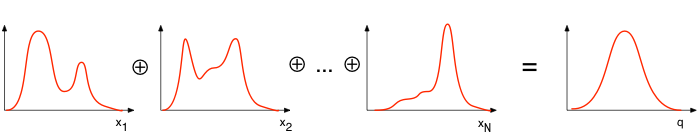
\includegraphics{Central_limit_theorem.png}
\caption{}
\end{figure}

Moreover, the central limit theorem states that the mean value of \(q\)
is given by

\begin{equation}
\mu_{q} = \sum_{i=1}^{N} \mu_{x_i} 
\end{equation}

and the variance (standard deviation squared) is given by

\begin{equation}
\sigma_{q}^{2} = \sum_{i=1}^{N} \sigma^2_{x_i} 
\end{equation}

\emph{if you are having problems with the math displaing, click
\href{http://nbviewer.jupyter.org/github/cranmer/intro-exp-phys-II/blob/master/Central-Limit-Theorem.ipynb?flush_cache=true}{here}}

The mean probably isn't surprising because \(q\) is just a sum and the
integral the defines the mean just distributes across each term. Also,
the equation for the variance is the same as the propagation of errors
formula we use when we add different measurements together. However,
that propoagation of errors formula is derived from the Central Limit
Theorem, not vice versa.

\subsubsection{This is a collaborative
project}\label{this-is-a-collaborative-project}

In this repository there is a folder called \texttt{distributions} with
several python files. The idea is that each student will create one of
these python files and we will use GitHub to collect them. Each of these
files has a python class that describes a probability distribution. Each
of these classes will define: * \texttt{x\_min,\ x\_max,\ f\_max} - used
for the accept/reject Monte Carlo sampling algorithm * \texttt{pdf()} -
the probability density function * \texttt{mean()} - the mean of the pdf
* \texttt{std()} - the standard deviation of the pdf

In addition, each of these python classes inherits from
\texttt{BaseDistribution} which knows how to run the accept/reject
algorithm using the information above
(\href{distributions/base_distribution.py}{see inside} ). In order to
generate \texttt{n\_samples} from the pdf, you simply call
\texttt{dist.rvs(n\_samples)}, where \texttt{dist} is an instance of one
of these python classes.

\textbf{Naming Convention}: Name your file
\texttt{Dist\_\textless{}netid\textgreater{}.py} and your distribution
the same way (without the \texttt{.py}). If you want to contribute more
than one distribution, you can can add
\texttt{Dist\_\textless{}netid\textgreater{}\_\textless{}index\textgreater{}.py},
where \texttt{\textless{}index\textgreater{}} is 1,2,3,...

Here's an example:

    \begin{Verbatim}[commandchars=\\\{\}]
{\color{incolor}In [{\color{incolor}26}]:} \PY{o}{!}cat distributions/Dist\PYZus{}kc90.py
\end{Verbatim}


    \begin{Verbatim}[commandchars=\\\{\}]
import numpy as np
from .base\_distribution import BaseDistribution

class Dist\_kc90(BaseDistribution):
	def \_\_init\_\_(self):
		self.f\_max = 1
		self.x\_min = -1
		self.x\_max = 1


	def pdf(self, x):
		"""This is your PDF"""
		return np.abs(x)

	def mean(self):
		"""This is the mean of the PDF"""
		return 0.

	def std(self):
		"""This is the standard deviation of the pdf"""
		return np.sqrt(0.5)



    \end{Verbatim}

    \section{Part 1: Create your distribution Send pull
request}\label{part-1-create-your-distribution-send-pull-request}

Basically everyone has done this by now. The master branch of the
repository has all the contributions

\section{Part 2: Pull the distribution to get all the contributed
Distributions}\label{part-2-pull-the-distribution-to-get-all-the-contributed-distributions}

Create a new branch called \texttt{part\ 2} from the master branch:

\begin{enumerate}
\def\labelenumi{\arabic{enumi}.}
\tightlist
\item
  First change to the master branch
\item
  Second create new branch
\end{enumerate}

Then, you need to open a shell (eg. from GitHub desktop you can:

\begin{itemize}
\tightlist
\item
  Windows:
  \texttt{Repository\ \textgreater{}\ Open\ in\ Command\ Prompt}
\item
  Mac: \texttt{Repository\ \textgreater{}\ Open\ in\ Terminal}
\end{itemize}

Then type: \texttt{git\ pull\ upstream\ master}

Now you should have many new distributions.

\section{Part 3: Update and Execute this
notebook.}\label{part-3-update-and-execute-this-notebook.}

The Cells labeled \texttt{In\ {[}10{]}} and \texttt{In\ {[}15{]}} refer
to the distributon \texttt{Dist\_kc90}. Update those lines to refer to
yoru distribution.

Then Execute the full notebook. \texttt{Cell\ \textgreater{}\ Run\ All}

    \begin{Verbatim}[commandchars=\\\{\}]
{\color{incolor}In [{\color{incolor}27}]:} \PY{k+kn}{from} \PY{n+nn}{datetime} \PY{k}{import} \PY{n}{date}
         \PY{n}{date}\PY{o}{.}\PY{n}{today}\PY{p}{(}\PY{p}{)}
\end{Verbatim}


\begin{Verbatim}[commandchars=\\\{\}]
{\color{outcolor}Out[{\color{outcolor}27}]:} datetime.date(2020, 5, 7)
\end{Verbatim}
            
    \subsection{Example usage of the
distributions}\label{example-usage-of-the-distributions}

Ok, now let's use them. So far there are only two distributions, but
there will be more soon.

    \begin{Verbatim}[commandchars=\\\{\}]
{\color{incolor}In [{\color{incolor}28}]:} \PY{o}{\PYZpc{}}\PY{k}{pylab} inline \PYZhy{}\PYZhy{}no\PYZhy{}import\PYZhy{}all
         \PY{k+kn}{from} \PY{n+nn}{scipy}\PY{n+nn}{.}\PY{n+nn}{stats} \PY{k}{import} \PY{n}{norm} \PY{c+c1}{\PYZsh{}will use this for plotting}
\end{Verbatim}


    \begin{Verbatim}[commandchars=\\\{\}]
Populating the interactive namespace from numpy and matplotlib

    \end{Verbatim}

    \begin{Verbatim}[commandchars=\\\{\}]
{\color{incolor}In [{\color{incolor}29}]:} \PY{c+c1}{\PYZsh{} import all our distributions}
         \PY{k+kn}{import} \PY{n+nn}{distributions}
\end{Verbatim}


    \begin{Verbatim}[commandchars=\\\{\}]
{\color{incolor}In [{\color{incolor}30}]:} \PY{c+c1}{\PYZsh{} some funny python to make a list of all the distributions for convenience}
         \PY{n}{all\PYZus{}distributions\PYZus{}dict} \PY{o}{=} \PY{n+nb}{dict}\PY{p}{(}\PY{p}{[}\PY{p}{(}\PY{n}{name}\PY{p}{,} \PY{n+nb+bp}{cls}\PY{p}{)} \PY{k}{for} \PY{n}{name}\PY{p}{,} \PY{n+nb+bp}{cls} \PY{o+ow}{in} \PY{n}{distributions}\PY{o}{.}\PY{n+nv+vm}{\PYZus{}\PYZus{}dict\PYZus{}\PYZus{}}\PY{o}{.}\PY{n}{items}\PY{p}{(}\PY{p}{)} \PY{k}{if} \PY{n+nb}{isinstance}\PY{p}{(}\PY{n+nb+bp}{cls}\PY{p}{,} \PY{n+nb}{type}\PY{p}{)}\PY{p}{]}\PY{p}{)}
         \PY{n}{all\PYZus{}distributions\PYZus{}list} \PY{o}{=} \PY{p}{[}\PY{p}{(}\PY{n+nb+bp}{cls}\PY{p}{)} \PY{k}{for} \PY{n}{name}\PY{p}{,} \PY{n+nb+bp}{cls} \PY{o+ow}{in} \PY{n}{distributions}\PY{o}{.}\PY{n+nv+vm}{\PYZus{}\PYZus{}dict\PYZus{}\PYZus{}}\PY{o}{.}\PY{n}{items}\PY{p}{(}\PY{p}{)} \PY{k}{if} \PY{n+nb}{isinstance}\PY{p}{(}\PY{n+nb+bp}{cls}\PY{p}{,} \PY{n+nb}{type}\PY{p}{)}\PY{p}{]}
         \PY{c+c1}{\PYZsh{} print out their names}
         \PY{n}{all\PYZus{}distributions\PYZus{}dict}\PY{o}{.}\PY{n}{keys}\PY{p}{(}\PY{p}{)}
\end{Verbatim}


\begin{Verbatim}[commandchars=\\\{\}]
{\color{outcolor}Out[{\color{outcolor}30}]:} dict\_keys(['Dist\_cmr653', 'Dist\_rdm445', 'Dist\_speedreed', 'Dist\_ltw244', 'Dist\_bt1369', 'Dist\_kc90', 'Dist\_rmr557', 'Dist\_jam1535', 'Dist\_at4227', 'Dist\_os852', 'Dist\_ia1113', 'Dist\_knd286', 'Dist\_aew492', 'Dist\_cah736', 'Dist\_phh250', 'Dist\_ks938', 'Dist\_sk7372', 'Dist\_kc90\_4', 'Dist\_sj2879', 'Dist\_dmc731', 'Dist\_sdl433', 'Dist\_pbg240', 'Dist\_pw1091', 'Dist\_lac683', 'Dist\_ajt540', 'Dist\_sm6779', 'Dist\_mkb452', 'Dist\_npl248', 'Dist\_speedreed2', 'Dist\_emm815', 'Dist\_yx1796', 'Dist\_abw400', 'Dist\_sea438', 'Dist\_sb6187', 'Dist\_ejt352', 'Dist\_tt1392', 'Dist\_jdg577'])
\end{Verbatim}
            
    \begin{Verbatim}[commandchars=\\\{\}]
{\color{incolor}In [{\color{incolor}31}]:} \PY{n+nb}{len}\PY{p}{(}\PY{n}{all\PYZus{}distributions\PYZus{}dict}\PY{o}{.}\PY{n}{keys}\PY{p}{(}\PY{p}{)}\PY{p}{)}
\end{Verbatim}


\begin{Verbatim}[commandchars=\\\{\}]
{\color{outcolor}Out[{\color{outcolor}31}]:} 37
\end{Verbatim}
            
    \begin{Verbatim}[commandchars=\\\{\}]
{\color{incolor}In [{\color{incolor}32}]:} \PY{c+c1}{\PYZsh{}\PYZsh{} Do tests}
         \PY{n}{ok\PYZus{}distributions\PYZus{}list}\PY{o}{=}\PY{p}{[}\PY{p}{]}
         \PY{n}{problems}\PY{o}{=}\PY{p}{[}\PY{p}{]}
         \PY{k}{for} \PY{n}{i}\PY{p}{,} \PY{n+nb+bp}{cls} \PY{o+ow}{in} \PY{n+nb}{enumerate}\PY{p}{(}\PY{n}{all\PYZus{}distributions\PYZus{}list}\PY{p}{)}\PY{p}{:}
             \PY{c+c1}{\PYZsh{}print(cls)}
             \PY{k}{try}\PY{p}{:}
                 \PY{n}{dist} \PY{o}{=} \PY{n+nb+bp}{cls}\PY{p}{(}\PY{p}{)}
                 \PY{n}{N\PYZus{}test} \PY{o}{=} \PY{l+m+mi}{10000}
                 \PY{c+c1}{\PYZsh{}print(\PYZsq{}will try to generate for \PYZpc{}s\PYZsq{} \PYZpc{}(cls.\PYZus{}\PYZus{}name\PYZus{}\PYZus{}))}
                 \PY{k}{if} \PY{n}{dist}\PY{o}{.}\PY{n}{pdf}\PY{p}{(}\PY{n}{dist}\PY{o}{.}\PY{n}{x\PYZus{}min} \PY{o}{+} \PY{o}{.}\PY{l+m+mi}{3}\PY{o}{*}\PY{p}{(}\PY{n}{dist}\PY{o}{.}\PY{n}{x\PYZus{}max}\PY{o}{\PYZhy{}}\PY{n}{dist}\PY{o}{.}\PY{n}{x\PYZus{}min}\PY{p}{)}\PY{p}{)} \PY{o}{\PYZlt{}} \PY{l+m+mf}{1E\PYZhy{}3}\PY{p}{:}
                     \PY{n+nb}{print}\PY{p}{(}\PY{l+s+s2}{\PYZdq{}}\PY{l+s+s2}{may have a problem}\PY{l+s+s2}{\PYZdq{}}\PY{p}{)}
                     \PY{k}{continue}
                     
                 \PY{n}{rvs} \PY{o}{=} \PY{n}{dist}\PY{o}{.}\PY{n}{rvs}\PY{p}{(}\PY{n}{N\PYZus{}test}\PY{p}{)}
                 \PY{k}{if} \PY{n}{np}\PY{o}{.}\PY{n}{abs}\PY{p}{(}\PY{n}{np}\PY{o}{.}\PY{n}{mean}\PY{p}{(}\PY{n}{rvs}\PY{p}{)} \PY{o}{\PYZhy{}} \PY{n}{dist}\PY{o}{.}\PY{n}{mean}\PY{p}{(}\PY{p}{)}\PY{p}{)} \PY{o}{\PYZgt{}} \PY{l+m+mi}{5}\PY{o}{*}\PY{n}{np}\PY{o}{.}\PY{n}{std}\PY{p}{(}\PY{n}{rvs}\PY{p}{)}\PY{o}{/}\PY{n}{np}\PY{o}{.}\PY{n}{sqrt}\PY{p}{(}\PY{n}{N\PYZus{}test}\PY{p}{)}\PY{p}{:}
                     \PY{n+nb}{print}\PY{p}{(}\PY{l+s+s2}{\PYZdq{}}\PY{l+s+s2}{means don}\PY{l+s+s2}{\PYZsq{}}\PY{l+s+s2}{t match for }\PY{l+s+si}{\PYZpc{}s}\PY{l+s+s2}{: }\PY{l+s+si}{\PYZpc{}f}\PY{l+s+s2}{ vs. }\PY{l+s+si}{\PYZpc{}f}\PY{l+s+s2}{\PYZdq{}} \PY{o}{\PYZpc{}}\PY{p}{(}\PY{n+nb+bp}{cls}\PY{o}{.}\PY{n+nv+vm}{\PYZus{}\PYZus{}name\PYZus{}\PYZus{}}\PY{p}{,} 
                                                                   \PY{n}{np}\PY{o}{.}\PY{n}{mean}\PY{p}{(}\PY{n}{rvs}\PY{p}{)}\PY{p}{,} \PY{n}{dist}\PY{o}{.}\PY{n}{mean}\PY{p}{(}\PY{p}{)}\PY{p}{)}\PY{p}{)}
                     \PY{k}{continue}
                     
                 \PY{k}{elif} \PY{n}{np}\PY{o}{.}\PY{n}{abs}\PY{p}{(}\PY{n}{np}\PY{o}{.}\PY{n}{std}\PY{p}{(}\PY{n}{rvs}\PY{p}{)} \PY{o}{\PYZhy{}} \PY{n}{dist}\PY{o}{.}\PY{n}{std}\PY{p}{(}\PY{p}{)}\PY{p}{)} \PY{o}{\PYZgt{}} \PY{l+m+mi}{5}\PY{o}{*}\PY{n}{np}\PY{o}{.}\PY{n}{std}\PY{p}{(}\PY{n}{rvs}\PY{p}{)}\PY{o}{/}\PY{n}{np}\PY{o}{.}\PY{n}{sqrt}\PY{p}{(}\PY{n}{np}\PY{o}{.}\PY{n}{sqrt}\PY{p}{(}\PY{l+m+mf}{1.}\PY{o}{*}\PY{n}{N\PYZus{}test}\PY{p}{)}\PY{p}{)}\PY{p}{:}
                     \PY{n+nb}{print}\PY{p}{(}\PY{l+s+s2}{\PYZdq{}}\PY{l+s+s2}{std devs. don}\PY{l+s+s2}{\PYZsq{}}\PY{l+s+s2}{t match for }\PY{l+s+si}{\PYZpc{}s}\PY{l+s+s2}{: }\PY{l+s+si}{\PYZpc{}f}\PY{l+s+s2}{ vs. }\PY{l+s+si}{\PYZpc{}f}\PY{l+s+s2}{\PYZdq{}} \PY{o}{\PYZpc{}}\PY{p}{(}\PY{n+nb+bp}{cls}\PY{o}{.}\PY{n+nv+vm}{\PYZus{}\PYZus{}name\PYZus{}\PYZus{}}\PY{p}{,} 
                                                                   \PY{n}{np}\PY{o}{.}\PY{n}{std}\PY{p}{(}\PY{n}{rvs}\PY{p}{)}\PY{p}{,} \PY{n}{dist}\PY{o}{.}\PY{n}{std}\PY{p}{(}\PY{p}{)}\PY{p}{)}\PY{p}{)}
                     \PY{k}{continue}
                 \PY{k}{elif} \PY{n}{np}\PY{o}{.}\PY{n}{abs}\PY{p}{(}\PY{n}{np}\PY{o}{.}\PY{n}{std}\PY{p}{(}\PY{n}{rvs}\PY{p}{)} \PY{o}{\PYZhy{}} \PY{n}{dist}\PY{o}{.}\PY{n}{std}\PY{p}{(}\PY{p}{)}\PY{p}{)} \PY{o}{/} \PY{n}{dist}\PY{o}{.}\PY{n}{std}\PY{p}{(}\PY{p}{)} \PY{o}{\PYZgt{}} \PY{l+m+mf}{0.1}\PY{p}{:}
                     \PY{n+nb}{print}\PY{p}{(}\PY{l+s+s2}{\PYZdq{}}\PY{l+s+s2}{std devs. don}\PY{l+s+s2}{\PYZsq{}}\PY{l+s+s2}{t match for }\PY{l+s+si}{\PYZpc{}s}\PY{l+s+s2}{: }\PY{l+s+si}{\PYZpc{}f}\PY{l+s+s2}{ vs. }\PY{l+s+si}{\PYZpc{}f}\PY{l+s+s2}{\PYZdq{}} \PY{o}{\PYZpc{}}\PY{p}{(}\PY{n+nb+bp}{cls}\PY{o}{.}\PY{n+nv+vm}{\PYZus{}\PYZus{}name\PYZus{}\PYZus{}}\PY{p}{,} 
                                                                   \PY{n}{np}\PY{o}{.}\PY{n}{std}\PY{p}{(}\PY{n}{rvs}\PY{p}{)}\PY{p}{,} \PY{n}{dist}\PY{o}{.}\PY{n}{std}\PY{p}{(}\PY{p}{)}\PY{p}{)}\PY{p}{)}
                     \PY{k}{continue}
                 
                 \PY{k}{elif} \PY{n}{np}\PY{o}{.}\PY{n}{sum}\PY{p}{(}\PY{n}{dist}\PY{o}{.}\PY{n}{pdf}\PY{p}{(}\PY{n}{np}\PY{o}{.}\PY{n}{linspace}\PY{p}{(}\PY{n}{dist}\PY{o}{.}\PY{n}{x\PYZus{}min}\PY{p}{,}\PY{n}{dist}\PY{o}{.}\PY{n}{x\PYZus{}max}\PY{p}{,}\PY{l+m+mi}{100}\PY{p}{)}\PY{p}{)}\PY{o}{\PYZlt{}}\PY{l+m+mi}{0}\PY{p}{)} \PY{o}{\PYZgt{}} \PY{l+m+mi}{0}\PY{p}{:}
                     \PY{n+nb}{print}\PY{p}{(}\PY{l+s+s2}{\PYZdq{}}\PY{l+s+s2}{pdf was negative in some places}\PY{l+s+s2}{\PYZdq{}}\PY{p}{)}
                     \PY{k}{continue}                    
         
                 \PY{k}{else}\PY{p}{:}
                     \PY{n+nb}{print}\PY{p}{(}\PY{l+s+s2}{\PYZdq{}}\PY{l+s+si}{\PYZpc{}s}\PY{l+s+s2}{ passes tests, adding it}\PY{l+s+s2}{\PYZdq{}} \PY{o}{\PYZpc{}}\PY{p}{(}\PY{n+nb+bp}{cls}\PY{o}{.}\PY{n+nv+vm}{\PYZus{}\PYZus{}name\PYZus{}\PYZus{}}\PY{p}{)}\PY{p}{)}
                     \PY{n}{ok\PYZus{}distributions\PYZus{}list}\PY{o}{.}\PY{n}{append}\PY{p}{(}\PY{n+nb+bp}{cls}\PY{p}{)}
             \PY{k}{except}\PY{p}{:}
                 \PY{n+nb}{print}\PY{p}{(}\PY{l+s+s2}{\PYZdq{}}\PY{l+s+si}{\PYZpc{}s}\PY{l+s+s2}{ has errors, does}\PY{l+s+s2}{\PYZsq{}}\PY{l+s+s2}{t work}\PY{l+s+s2}{\PYZdq{}} \PY{o}{\PYZpc{}}\PY{p}{(}\PY{n+nb+bp}{cls}\PY{o}{.}\PY{n+nv+vm}{\PYZus{}\PYZus{}name\PYZus{}\PYZus{}}\PY{p}{)}\PY{p}{)}
                 \PY{k}{continue}
         
         \PY{n+nb}{print}\PY{p}{(}\PY{l+s+s2}{\PYZdq{}}\PY{l+s+s2}{list of ok distributions:}\PY{l+s+s2}{\PYZdq{}}\PY{p}{,}\PY{p}{[}\PY{n}{i}\PY{o}{.}\PY{n+nv+vm}{\PYZus{}\PYZus{}name\PYZus{}\PYZus{}} \PY{k}{for} \PY{n}{i} \PY{o+ow}{in} \PY{n}{ok\PYZus{}distributions\PYZus{}list}\PY{p}{]}\PY{p}{)}
\end{Verbatim}


    \begin{Verbatim}[commandchars=\\\{\}]
Dist\_cmr653 passes tests, adding it
Dist\_rdm445 passes tests, adding it
Dist\_speedreed passes tests, adding it
Dist\_ltw244 passes tests, adding it
Dist\_bt1369 passes tests, adding it
Dist\_kc90 passes tests, adding it
Dist\_rmr557 passes tests, adding it
Dist\_jam1535 has errors, does't work
Dist\_at4227 passes tests, adding it
Dist\_os852 passes tests, adding it
Dist\_ia1113 passes tests, adding it
Dist\_knd286 passes tests, adding it
Dist\_aew492 passes tests, adding it

    \end{Verbatim}

    \begin{Verbatim}[commandchars=\\\{\}]
/Users/mariekazburns/Documents/GitHub/intro-exp-phys-II/distributions/Dist\_cah736.py:13: RuntimeWarning: invalid value encountered in true\_divide
  return ((np.sin(x)**2))/(1.55595*x)
/Users/mariekazburns/anaconda3/lib/python3.6/site-packages/ipykernel\_launcher.py:29: RuntimeWarning: invalid value encountered in less

    \end{Verbatim}

    \begin{Verbatim}[commandchars=\\\{\}]
Dist\_cah736 passes tests, adding it
Dist\_phh250 passes tests, adding it
Dist\_ks938 passes tests, adding it
Dist\_sk7372 passes tests, adding it
Dist\_kc90\_4 passes tests, adding it
Dist\_sj2879 passes tests, adding it
Dist\_dmc731 passes tests, adding it
Dist\_sdl433 passes tests, adding it
means don't match for Dist\_pbg240: 2.413056 vs. 3.200000
Dist\_pw1091 passes tests, adding it
Dist\_lac683 passes tests, adding it
Dist\_ajt540 passes tests, adding it
Dist\_sm6779 passes tests, adding it
means don't match for Dist\_mkb452: 2.070212 vs. 2.066190
Dist\_npl248 passes tests, adding it
Dist\_speedreed2 passes tests, adding it
Dist\_emm815 passes tests, adding it
Dist\_yx1796 passes tests, adding it
Dist\_abw400 passes tests, adding it
Dist\_sea438 passes tests, adding it
Dist\_sb6187 passes tests, adding it
Dist\_ejt352 passes tests, adding it
Dist\_tt1392 passes tests, adding it
Dist\_jdg577 passes tests, adding it
list of ok distributions: ['Dist\_cmr653', 'Dist\_rdm445', 'Dist\_speedreed', 'Dist\_ltw244', 'Dist\_bt1369', 'Dist\_kc90', 'Dist\_rmr557', 'Dist\_at4227', 'Dist\_os852', 'Dist\_ia1113', 'Dist\_knd286', 'Dist\_aew492', 'Dist\_cah736', 'Dist\_phh250', 'Dist\_ks938', 'Dist\_sk7372', 'Dist\_kc90\_4', 'Dist\_sj2879', 'Dist\_dmc731', 'Dist\_sdl433', 'Dist\_pw1091', 'Dist\_lac683', 'Dist\_ajt540', 'Dist\_sm6779', 'Dist\_npl248', 'Dist\_speedreed2', 'Dist\_emm815', 'Dist\_yx1796', 'Dist\_abw400', 'Dist\_sea438', 'Dist\_sb6187', 'Dist\_ejt352', 'Dist\_tt1392', 'Dist\_jdg577']

    \end{Verbatim}

    \begin{Verbatim}[commandchars=\\\{\}]
{\color{incolor}In [{\color{incolor}33}]:} \PY{n}{problems} \PY{o}{=} \PY{p}{[}\PY{n}{x} \PY{k}{for} \PY{n}{x} \PY{o+ow}{in} \PY{n}{all\PYZus{}distributions\PYZus{}list} \PY{k}{if} \PY{n}{x} \PY{o+ow}{not} \PY{o+ow}{in} \PY{n}{ok\PYZus{}distributions\PYZus{}list}\PY{p}{]}
         \PY{p}{[}\PY{n}{i}\PY{o}{.}\PY{n+nv+vm}{\PYZus{}\PYZus{}name\PYZus{}\PYZus{}} \PY{k}{for} \PY{n}{i} \PY{o+ow}{in} \PY{n}{problems}\PY{p}{]}
\end{Verbatim}


\begin{Verbatim}[commandchars=\\\{\}]
{\color{outcolor}Out[{\color{outcolor}33}]:} ['Dist\_jam1535', 'Dist\_pbg240', 'Dist\_mkb452']
\end{Verbatim}
            
    \begin{Verbatim}[commandchars=\\\{\}]
{\color{incolor}In [{\color{incolor}34}]:} \PY{c+c1}{\PYZsh{} how many samples for plots?}
         \PY{n}{n\PYZus{}samples} \PY{o}{=} \PY{l+m+mi}{100000}
\end{Verbatim}


    \textbf{Update to use your distribution}

    \begin{Verbatim}[commandchars=\\\{\}]
{\color{incolor}In [{\color{incolor}35}]:} \PY{c+c1}{\PYZsh{} Here\PYZsq{}s an example of usage}
         \PY{n}{dist} \PY{o}{=} \PY{n}{distributions}\PY{o}{.}\PY{n}{Dist\PYZus{}mkb452}\PY{p}{(}\PY{p}{)}
         \PY{n}{rvs} \PY{o}{=} \PY{n}{dist}\PY{o}{.}\PY{n}{rvs}\PY{p}{(}\PY{n}{n\PYZus{}samples}\PY{p}{)}
         \PY{n}{counts}\PY{p}{,} \PY{n}{bins}\PY{p}{,} \PY{n}{edges} \PY{o}{=} \PY{n}{plt}\PY{o}{.}\PY{n}{hist}\PY{p}{(}\PY{n}{rvs}\PY{p}{,} \PY{n}{bins}\PY{o}{=}\PY{l+m+mi}{50}\PY{p}{,} \PY{n}{density}\PY{o}{=}\PY{k+kc}{True}\PY{p}{,} \PY{n}{alpha} \PY{o}{=}\PY{l+m+mf}{0.2}\PY{p}{)}
         \PY{n}{y} \PY{o}{=} \PY{p}{[}\PY{p}{]}
         \PY{k}{for} \PY{n+nb}{bin} \PY{o+ow}{in} \PY{n}{bins}\PY{p}{:}
             \PY{n}{y}\PY{o}{.}\PY{n}{append}\PY{p}{(}\PY{n}{dist}\PY{o}{.}\PY{n}{pdf}\PY{p}{(}\PY{n+nb}{bin}\PY{p}{)}\PY{p}{)}
         \PY{n}{plt}\PY{o}{.}\PY{n}{plot}\PY{p}{(}\PY{n}{bins}\PY{p}{,} \PY{n}{y}\PY{p}{,} \PY{n}{c}\PY{o}{=}\PY{l+s+s1}{\PYZsq{}}\PY{l+s+s1}{r}\PY{l+s+s1}{\PYZsq{}}\PY{p}{,} \PY{n}{lw}\PY{o}{=}\PY{l+m+mi}{2}\PY{p}{)}
\end{Verbatim}


\begin{Verbatim}[commandchars=\\\{\}]
{\color{outcolor}Out[{\color{outcolor}35}]:} [<matplotlib.lines.Line2D at 0x1a20391048>]
\end{Verbatim}
            
    \begin{center}
    \adjustimage{max size={0.9\linewidth}{0.9\paperheight}}{output_13_1.png}
    \end{center}
    { \hspace*{\fill} \\}
    
    \begin{Verbatim}[commandchars=\\\{\}]
{\color{incolor}In [{\color{incolor}36}]:} \PY{n}{dist}\PY{o}{.}\PY{n}{std}\PY{p}{(}\PY{p}{)}
\end{Verbatim}


\begin{Verbatim}[commandchars=\\\{\}]
{\color{outcolor}Out[{\color{outcolor}36}]:} 0.06436
\end{Verbatim}
            
    \subsection{Let's inspect all the distributions we
have}\label{lets-inspect-all-the-distributions-we-have}

Here we will loop over the different distributions and make a plot like
the one above

    \begin{Verbatim}[commandchars=\\\{\}]
{\color{incolor}In [{\color{incolor}37}]:} \PY{n}{fig} \PY{o}{=} \PY{n}{plt}\PY{o}{.}\PY{n}{figure}\PY{p}{(}\PY{n}{figsize}\PY{o}{=}\PY{l+m+mi}{2}\PY{o}{*}\PY{n}{plt}\PY{o}{.}\PY{n}{figaspect}\PY{p}{(}\PY{n+nb}{len}\PY{p}{(}\PY{n}{ok\PYZus{}distributions\PYZus{}list}\PY{p}{)}\PY{p}{)}\PY{p}{)}
         \PY{k}{for} \PY{n}{i}\PY{p}{,} \PY{n+nb+bp}{cls} \PY{o+ow}{in} \PY{n+nb}{enumerate}\PY{p}{(}\PY{n}{ok\PYZus{}distributions\PYZus{}list}\PY{p}{)}\PY{p}{:}
             \PY{n}{dist} \PY{o}{=} \PY{n+nb+bp}{cls}\PY{p}{(}\PY{p}{)}
             \PY{n}{rvs} \PY{o}{=} \PY{n}{dist}\PY{o}{.}\PY{n}{rvs}\PY{p}{(}\PY{l+m+mi}{10000}\PY{p}{)}
             \PY{n}{ax} \PY{o}{=} \PY{n}{fig}\PY{o}{.}\PY{n}{add\PYZus{}subplot}\PY{p}{(}\PY{n+nb}{len}\PY{p}{(}\PY{n}{ok\PYZus{}distributions\PYZus{}list}\PY{p}{)}\PY{p}{,}\PY{l+m+mi}{1}\PY{p}{,}\PY{n}{i}\PY{o}{+}\PY{l+m+mi}{1}\PY{p}{)}
             \PY{n}{counts}\PY{p}{,} \PY{n}{bins}\PY{p}{,} \PY{n}{patches} \PY{o}{=} \PY{n}{ax}\PY{o}{.}\PY{n}{hist}\PY{p}{(}\PY{n}{rvs}\PY{p}{,} \PY{n}{bins}\PY{o}{=}\PY{l+m+mi}{50}\PY{p}{,} \PY{n}{density}\PY{o}{=}\PY{k+kc}{True}\PY{p}{,} \PY{n}{alpha}\PY{o}{=}\PY{l+m+mf}{0.2}\PY{p}{)}
             \PY{c+c1}{\PYZsh{} depending on how you code up your pdf() function, numpy might not}
             \PY{c+c1}{\PYZsh{} be able to \PYZdq{}broadcast\PYZdq{} (apply the function for each element of a numpy array)}
             \PY{c+c1}{\PYZsh{} but this should always wrok}
             \PY{n}{y} \PY{o}{=} \PY{p}{[}\PY{p}{]}
             \PY{k}{for} \PY{n+nb}{bin} \PY{o+ow}{in} \PY{n}{bins}\PY{p}{:}
                 \PY{n}{y}\PY{o}{.}\PY{n}{append}\PY{p}{(}\PY{n}{dist}\PY{o}{.}\PY{n}{pdf}\PY{p}{(}\PY{n+nb}{bin}\PY{p}{)}\PY{p}{)}
                 
             \PY{c+c1}{\PYZsh{} ok, now plot it}
             \PY{n}{plt}\PY{o}{.}\PY{n}{plot}\PY{p}{(}\PY{n}{bins}\PY{p}{,} \PY{n}{y}\PY{p}{,} \PY{n}{c}\PY{o}{=}\PY{l+s+s1}{\PYZsq{}}\PY{l+s+s1}{r}\PY{l+s+s1}{\PYZsq{}}\PY{p}{,} \PY{n}{lw}\PY{o}{=}\PY{l+m+mi}{2}\PY{p}{)}
             
             \PY{c+c1}{\PYZsh{} and let\PYZsq{}s check if the distribution is ok}
             \PY{n+nb}{print}\PY{p}{(}\PY{l+s+s2}{\PYZdq{}}\PY{l+s+si}{\PYZpc{}s}\PY{l+s+s2}{: std from samples = }\PY{l+s+si}{\PYZpc{}.2f}\PY{l+s+s2}{, std from dist = }\PY{l+s+si}{\PYZpc{}.2f}\PY{l+s+s2}{\PYZdq{}} \PY{o}{\PYZpc{}}\PY{p}{(}\PY{n+nb+bp}{cls}\PY{o}{.}\PY{n+nv+vm}{\PYZus{}\PYZus{}name\PYZus{}\PYZus{}}\PY{p}{,}\PY{n}{np}\PY{o}{.}\PY{n}{std}\PY{p}{(}\PY{n}{dist}\PY{o}{.}\PY{n}{rvs}\PY{p}{(}\PY{n}{n\PYZus{}samples}\PY{p}{)}\PY{p}{)}\PY{p}{,} \PY{n}{dist}\PY{o}{.}\PY{n}{std}\PY{p}{(}\PY{p}{)}\PY{p}{)}\PY{p}{)}
             \PY{k}{if} \PY{n}{np}\PY{o}{.}\PY{n}{abs}\PY{p}{(}\PY{n}{np}\PY{o}{.}\PY{n}{std}\PY{p}{(}\PY{n}{dist}\PY{o}{.}\PY{n}{rvs}\PY{p}{(}\PY{n}{n\PYZus{}samples}\PY{p}{)}\PY{p}{)} \PY{o}{\PYZhy{}} \PY{n}{dist}\PY{o}{.}\PY{n}{std}\PY{p}{(}\PY{p}{)}\PY{p}{)} \PY{o}{/} \PY{n}{dist}\PY{o}{.}\PY{n}{std}\PY{p}{(}\PY{p}{)} \PY{o}{\PYZgt{}} \PY{l+m+mf}{0.1}\PY{p}{:}
                 \PY{n+nb}{print}\PY{p}{(}\PY{l+s+s2}{\PYZdq{}}\PY{l+s+s2}{looks like a problem with this distribution: }\PY{l+s+s2}{\PYZdq{}}\PY{p}{,} \PY{n+nb+bp}{cls}\PY{p}{)}
\end{Verbatim}


    \begin{Verbatim}[commandchars=\\\{\}]
Dist\_cmr653: std from samples = 1.25, std from dist = 1.25
Dist\_rdm445: std from samples = 0.71, std from dist = 0.71
Dist\_speedreed: std from samples = 1.41, std from dist = 1.41
Dist\_ltw244: std from samples = 0.58, std from dist = 0.58
Dist\_bt1369: std from samples = 1.57, std from dist = 1.57
Dist\_kc90: std from samples = 0.71, std from dist = 0.71
Dist\_rmr557: std from samples = 0.61, std from dist = 0.61
Dist\_at4227: std from samples = 0.68, std from dist = 0.68
Dist\_os852: std from samples = 0.65, std from dist = 0.65
Dist\_ia1113: std from samples = 0.14, std from dist = 0.14
Dist\_knd286: std from samples = 0.31, std from dist = 0.31
Dist\_aew492: std from samples = 0.39, std from dist = 0.39
Dist\_cah736: std from samples = 1.50, std from dist = 1.50
Dist\_phh250: std from samples = 0.24, std from dist = 0.24
Dist\_ks938: std from samples = 0.71, std from dist = 0.71
Dist\_sk7372: std from samples = 0.77, std from dist = 0.77
Dist\_kc90\_4: std from samples = 0.71, std from dist = 0.71
Dist\_sj2879: std from samples = 2.33, std from dist = 2.32
Dist\_dmc731: std from samples = 0.69, std from dist = 0.70
Dist\_sdl433: std from samples = 0.39, std from dist = 0.39
Dist\_pw1091: std from samples = 0.88, std from dist = 0.89
Dist\_lac683: std from samples = 0.58, std from dist = 0.54
Dist\_ajt540: std from samples = 0.17, std from dist = 0.17
Dist\_sm6779: std from samples = 0.28, std from dist = 0.28
Dist\_npl248: std from samples = 0.71, std from dist = 0.71
Dist\_speedreed2: std from samples = 1.41, std from dist = 1.41
Dist\_emm815: std from samples = 0.19, std from dist = 0.19
Dist\_yx1796: std from samples = 0.52, std from dist = 0.52
Dist\_abw400: std from samples = 0.26, std from dist = 0.26
Dist\_sea438: std from samples = 0.71, std from dist = 0.71
Dist\_sb6187: std from samples = 1.90, std from dist = 1.90
Dist\_ejt352: std from samples = 0.71, std from dist = 0.71
Dist\_tt1392: std from samples = 0.71, std from dist = 0.71
Dist\_jdg577: std from samples = 0.71, std from dist = 0.71

    \end{Verbatim}

    \begin{center}
    \adjustimage{max size={0.9\linewidth}{0.9\paperheight}}{output_16_1.png}
    \end{center}
    { \hspace*{\fill} \\}
    
    \begin{Verbatim}[commandchars=\\\{\}]
{\color{incolor}In [{\color{incolor}38}]:} \PY{n}{fig} \PY{o}{=} \PY{n}{plt}\PY{o}{.}\PY{n}{figure}\PY{p}{(}\PY{n}{figsize}\PY{o}{=}\PY{l+m+mi}{2}\PY{o}{*}\PY{n}{plt}\PY{o}{.}\PY{n}{figaspect}\PY{p}{(}\PY{n+nb}{len}\PY{p}{(}\PY{n}{problems}\PY{p}{)}\PY{p}{)}\PY{p}{)}
         \PY{k}{for} \PY{n}{i}\PY{p}{,} \PY{n+nb+bp}{cls} \PY{o+ow}{in} \PY{n+nb}{enumerate}\PY{p}{(}\PY{n}{problems}\PY{p}{)}\PY{p}{:}
             \PY{n}{dist} \PY{o}{=} \PY{n+nb+bp}{cls}\PY{p}{(}\PY{p}{)}
             \PY{n}{rvs} \PY{o}{=} \PY{n}{dist}\PY{o}{.}\PY{n}{rvs}\PY{p}{(}\PY{l+m+mi}{10000}\PY{p}{)}
             \PY{n}{ax} \PY{o}{=} \PY{n}{fig}\PY{o}{.}\PY{n}{add\PYZus{}subplot}\PY{p}{(}\PY{n+nb}{len}\PY{p}{(}\PY{n}{ok\PYZus{}distributions\PYZus{}list}\PY{p}{)}\PY{p}{,}\PY{l+m+mi}{1}\PY{p}{,}\PY{n}{i}\PY{o}{+}\PY{l+m+mi}{1}\PY{p}{)}
             \PY{n}{counts}\PY{p}{,} \PY{n}{bins}\PY{p}{,} \PY{n}{patches} \PY{o}{=} \PY{n}{ax}\PY{o}{.}\PY{n}{hist}\PY{p}{(}\PY{n}{rvs}\PY{p}{,} \PY{n}{bins}\PY{o}{=}\PY{l+m+mi}{50}\PY{p}{,} \PY{n}{density}\PY{o}{=}\PY{k+kc}{True}\PY{p}{,} \PY{n}{alpha}\PY{o}{=}\PY{l+m+mf}{0.2}\PY{p}{)}
             \PY{c+c1}{\PYZsh{} depending on how you code up your pdf() function, numpy might not}
             \PY{c+c1}{\PYZsh{} be able to \PYZdq{}broadcast\PYZdq{} (apply the function for each element of a numpy array)}
             \PY{c+c1}{\PYZsh{} but this should always wrok}
             \PY{n}{y} \PY{o}{=} \PY{p}{[}\PY{p}{]}
             \PY{k}{for} \PY{n+nb}{bin} \PY{o+ow}{in} \PY{n}{bins}\PY{p}{:}
                 \PY{n}{y}\PY{o}{.}\PY{n}{append}\PY{p}{(}\PY{n}{dist}\PY{o}{.}\PY{n}{pdf}\PY{p}{(}\PY{n+nb}{bin}\PY{p}{)}\PY{p}{)}
                 
             \PY{c+c1}{\PYZsh{} ok, now plot it}
             \PY{n}{plt}\PY{o}{.}\PY{n}{plot}\PY{p}{(}\PY{n}{bins}\PY{p}{,} \PY{n}{y}\PY{p}{,} \PY{n}{c}\PY{o}{=}\PY{l+s+s1}{\PYZsq{}}\PY{l+s+s1}{r}\PY{l+s+s1}{\PYZsq{}}\PY{p}{,} \PY{n}{lw}\PY{o}{=}\PY{l+m+mi}{2}\PY{p}{)}
             
             \PY{c+c1}{\PYZsh{} and let\PYZsq{}s check if the distribution is ok}
             \PY{n+nb}{print}\PY{p}{(}\PY{l+s+s2}{\PYZdq{}}\PY{l+s+si}{\PYZpc{}s}\PY{l+s+s2}{: std from samples = }\PY{l+s+si}{\PYZpc{}.2f}\PY{l+s+s2}{, std from dist = }\PY{l+s+si}{\PYZpc{}.2f}\PY{l+s+s2}{\PYZdq{}} \PY{o}{\PYZpc{}}\PY{p}{(}\PY{n+nb+bp}{cls}\PY{o}{.}\PY{n+nv+vm}{\PYZus{}\PYZus{}name\PYZus{}\PYZus{}}\PY{p}{,}\PY{n}{np}\PY{o}{.}\PY{n}{std}\PY{p}{(}\PY{n}{dist}\PY{o}{.}\PY{n}{rvs}\PY{p}{(}\PY{n}{n\PYZus{}samples}\PY{p}{)}\PY{p}{)}\PY{p}{,} \PY{n}{dist}\PY{o}{.}\PY{n}{std}\PY{p}{(}\PY{p}{)}\PY{p}{)}\PY{p}{)}
             \PY{k}{if} \PY{n}{np}\PY{o}{.}\PY{n}{abs}\PY{p}{(}\PY{n}{np}\PY{o}{.}\PY{n}{std}\PY{p}{(}\PY{n}{dist}\PY{o}{.}\PY{n}{rvs}\PY{p}{(}\PY{n}{n\PYZus{}samples}\PY{p}{)}\PY{p}{)} \PY{o}{\PYZhy{}} \PY{n}{dist}\PY{o}{.}\PY{n}{std}\PY{p}{(}\PY{p}{)}\PY{p}{)} \PY{o}{/} \PY{n}{dist}\PY{o}{.}\PY{n}{std}\PY{p}{(}\PY{p}{)} \PY{o}{\PYZgt{}} \PY{l+m+mf}{0.1}\PY{p}{:}
                 \PY{n+nb}{print}\PY{p}{(}\PY{l+s+s2}{\PYZdq{}}\PY{l+s+s2}{looks like a problem with this distribution: }\PY{l+s+s2}{\PYZdq{}}\PY{p}{,} \PY{n+nb+bp}{cls}\PY{p}{)}
\end{Verbatim}


    \begin{Verbatim}[commandchars=\\\{\}]
Dist\_jam1535: std from samples = 0.84, std from dist = 0.84
Dist\_pbg240: std from samples = 1.05, std from dist = 9.26
looks like a problem with this distribution:  <class 'distributions.Dist\_pbg240.Dist\_pbg240'>
Dist\_mkb452: std from samples = 0.06, std from dist = 0.06

    \end{Verbatim}

    \begin{center}
    \adjustimage{max size={0.9\linewidth}{0.9\paperheight}}{output_17_1.png}
    \end{center}
    { \hspace*{\fill} \\}
    
    \subsection{Demonstration of the Central Limit
Theorem}\label{demonstration-of-the-central-limit-theorem}

ok, let's use one of the distributions to demonstrate the central limit
theorem. We will use the same distribution \(N\) times.

First let's make a little helper function.

    \begin{Verbatim}[commandchars=\\\{\}]
{\color{incolor}In [{\color{incolor}39}]:} \PY{k}{def} \PY{n+nf}{do\PYZus{}convolution}\PY{p}{(}\PY{n}{dist}\PY{p}{,} \PY{n}{N}\PY{p}{)}\PY{p}{:}
             \PY{n}{n\PYZus{}samples} \PY{o}{=} \PY{l+m+mi}{10000}
             \PY{n}{q} \PY{o}{=} \PY{n}{np}\PY{o}{.}\PY{n}{zeros}\PY{p}{(}\PY{n}{n\PYZus{}samples}\PY{p}{)}
             \PY{n}{var\PYZus{}q} \PY{o}{=} \PY{l+m+mf}{0.}
             \PY{n}{mean\PYZus{}q} \PY{o}{=} \PY{l+m+mf}{0.}
         
             \PY{k}{for} \PY{n}{i} \PY{o+ow}{in} \PY{n+nb}{range}\PY{p}{(}\PY{n}{N}\PY{p}{)}\PY{p}{:}
                 \PY{n}{q} \PY{o}{=} \PY{n}{q}\PY{o}{+}\PY{n}{dist}\PY{o}{.}\PY{n}{rvs}\PY{p}{(}\PY{n}{n\PYZus{}samples}\PY{p}{)}
                 \PY{n}{var\PYZus{}q} \PY{o}{=} \PY{n}{var\PYZus{}q} \PY{o}{+} \PY{n}{dist}\PY{o}{.}\PY{n}{std}\PY{p}{(}\PY{p}{)}\PY{o}{*}\PY{o}{*}\PY{l+m+mi}{2}
                 \PY{n}{mean\PYZus{}q} \PY{o}{=} \PY{n}{mean\PYZus{}q} \PY{o}{+} \PY{n}{dist}\PY{o}{.}\PY{n}{mean}\PY{p}{(}\PY{p}{)}
         
             \PY{n}{std\PYZus{}q} \PY{o}{=} \PY{n}{np}\PY{o}{.}\PY{n}{sqrt}\PY{p}{(} \PY{n}{var\PYZus{}q} \PY{p}{)}
         
         
             \PY{n}{counts}\PY{p}{,} \PY{n}{bins}\PY{p}{,} \PY{n}{patches} \PY{o}{=} \PY{n}{plt}\PY{o}{.}\PY{n}{hist}\PY{p}{(}\PY{n}{q}\PY{p}{,}\PY{n}{bins}\PY{o}{=}\PY{l+m+mi}{50}\PY{p}{,} \PY{n}{density}\PY{o}{=}\PY{k+kc}{True}\PY{p}{,} \PY{n}{alpha}\PY{o}{=}\PY{o}{.}\PY{l+m+mi}{2}\PY{p}{)}
             \PY{n}{plt}\PY{o}{.}\PY{n}{plot}\PY{p}{(}\PY{n}{bins}\PY{p}{,} \PY{n}{norm}\PY{o}{.}\PY{n}{pdf}\PY{p}{(}\PY{n}{bins}\PY{p}{,}\PY{n}{loc}\PY{o}{=}\PY{n}{mean\PYZus{}q}\PY{p}{,} \PY{n}{scale}\PY{o}{=}\PY{n}{std\PYZus{}q}\PY{p}{)}\PY{p}{,} \PY{n}{lw}\PY{o}{=}\PY{l+m+mi}{2}\PY{p}{,} \PY{n}{c}\PY{o}{=}\PY{l+s+s1}{\PYZsq{}}\PY{l+s+s1}{r}\PY{l+s+s1}{\PYZsq{}}\PY{p}{)}
\end{Verbatim}


    Now let's use it for \(N=\{2,4,32\}\)

\textbf{UPDATE THE NEXT LINE TO USE YOUR DISTRIBUTION}

    \begin{Verbatim}[commandchars=\\\{\}]
{\color{incolor}In [{\color{incolor}40}]:} \PY{n}{dist} \PY{o}{=} \PY{n}{distributions}\PY{o}{.}\PY{n}{Dist\PYZus{}mkb452}\PY{p}{(}\PY{p}{)}  \PY{c+c1}{\PYZsh{}update me!}
         \PY{n}{do\PYZus{}convolution}\PY{p}{(}\PY{n}{dist}\PY{p}{,}\PY{l+m+mi}{2}\PY{p}{)}
\end{Verbatim}


    \begin{center}
    \adjustimage{max size={0.9\linewidth}{0.9\paperheight}}{output_21_0.png}
    \end{center}
    { \hspace*{\fill} \\}
    
    \begin{Verbatim}[commandchars=\\\{\}]
{\color{incolor}In [{\color{incolor}41}]:} \PY{n}{do\PYZus{}convolution}\PY{p}{(}\PY{n}{dist}\PY{p}{,}\PY{l+m+mi}{4}\PY{p}{)}
\end{Verbatim}


    \begin{center}
    \adjustimage{max size={0.9\linewidth}{0.9\paperheight}}{output_22_0.png}
    \end{center}
    { \hspace*{\fill} \\}
    
    \begin{Verbatim}[commandchars=\\\{\}]
{\color{incolor}In [{\color{incolor}42}]:} \PY{n}{do\PYZus{}convolution}\PY{p}{(}\PY{n}{dist}\PY{p}{,}\PY{l+m+mi}{32}\PY{p}{)}
\end{Verbatim}


    \begin{center}
    \adjustimage{max size={0.9\linewidth}{0.9\paperheight}}{output_23_0.png}
    \end{center}
    { \hspace*{\fill} \\}
    
    \emph{Gorgeous!}

    \subsection{Now let's do the same thing randomly using different
distributions}\label{now-lets-do-the-same-thing-randomly-using-different-distributions}

To do this we will use \texttt{np.random.choice} to randomly choose from
our list. Here's an example

    \begin{Verbatim}[commandchars=\\\{\}]
{\color{incolor}In [{\color{incolor}43}]:} \PY{n}{np}\PY{o}{.}\PY{n}{random}\PY{o}{.}\PY{n}{choice}\PY{p}{(}\PY{p}{[}\PY{l+s+s1}{\PYZsq{}}\PY{l+s+s1}{a}\PY{l+s+s1}{\PYZsq{}}\PY{p}{,}\PY{l+s+s1}{\PYZsq{}}\PY{l+s+s1}{b}\PY{l+s+s1}{\PYZsq{}}\PY{p}{,}\PY{l+s+s1}{\PYZsq{}}\PY{l+s+s1}{c}\PY{l+s+s1}{\PYZsq{}}\PY{p}{,}\PY{l+s+s1}{\PYZsq{}}\PY{l+s+s1}{d}\PY{l+s+s1}{\PYZsq{}}\PY{p}{]}\PY{p}{,} \PY{l+m+mi}{10}\PY{p}{)}
\end{Verbatim}


\begin{Verbatim}[commandchars=\\\{\}]
{\color{outcolor}Out[{\color{outcolor}43}]:} array(['b', 'd', 'b', 'b', 'a', 'a', 'b', 'd', 'a', 'd'], dtype='<U1')
\end{Verbatim}
            
    Now let's make a variation on the helper function above

    \begin{Verbatim}[commandchars=\\\{\}]
{\color{incolor}In [{\color{incolor}44}]:} \PY{k}{def} \PY{n+nf}{do\PYZus{}random\PYZus{}convolution}\PY{p}{(}\PY{n}{list\PYZus{}of\PYZus{}distributions}\PY{p}{,} \PY{n}{N}\PY{p}{)}\PY{p}{:}
             \PY{n}{n\PYZus{}samples} \PY{o}{=} \PY{l+m+mi}{10000}
             \PY{n}{q} \PY{o}{=} \PY{n}{np}\PY{o}{.}\PY{n}{zeros}\PY{p}{(}\PY{n}{n\PYZus{}samples}\PY{p}{)}
             \PY{n}{var\PYZus{}q} \PY{o}{=} \PY{l+m+mf}{0.}
             \PY{n}{mean\PYZus{}q} \PY{o}{=} \PY{l+m+mf}{0.}
         
             \PY{k}{for} \PY{n}{dist\PYZus{}class} \PY{o+ow}{in} \PY{n}{np}\PY{o}{.}\PY{n}{random}\PY{o}{.}\PY{n}{choice}\PY{p}{(}\PY{n}{list\PYZus{}of\PYZus{}distributions}\PY{p}{,}\PY{n}{N}\PY{p}{)}\PY{p}{:}
                 \PY{n}{dist} \PY{o}{=} \PY{n}{dist\PYZus{}class}\PY{p}{(}\PY{p}{)}
                 \PY{n+nb}{print}\PY{p}{(}\PY{n}{dist\PYZus{}class}\PY{o}{.}\PY{n+nv+vm}{\PYZus{}\PYZus{}name\PYZus{}\PYZus{}}\PY{p}{,} \PY{n}{dist}\PY{o}{.}\PY{n}{std}\PY{p}{(}\PY{p}{)}\PY{p}{)}
                 \PY{n}{q} \PY{o}{=} \PY{n}{q}\PY{o}{+}\PY{n}{dist}\PY{o}{.}\PY{n}{rvs}\PY{p}{(}\PY{n}{n\PYZus{}samples}\PY{p}{)}
                 \PY{n}{var\PYZus{}q} \PY{o}{=} \PY{n}{var\PYZus{}q} \PY{o}{+} \PY{n}{dist}\PY{o}{.}\PY{n}{std}\PY{p}{(}\PY{p}{)}\PY{o}{*}\PY{o}{*}\PY{l+m+mi}{2}
                 \PY{n}{mean\PYZus{}q} \PY{o}{=} \PY{n}{mean\PYZus{}q} \PY{o}{+} \PY{n}{dist}\PY{o}{.}\PY{n}{mean}\PY{p}{(}\PY{p}{)}
         
             \PY{n}{std\PYZus{}q} \PY{o}{=} \PY{n}{np}\PY{o}{.}\PY{n}{sqrt}\PY{p}{(} \PY{n}{var\PYZus{}q} \PY{p}{)}
         
         
             \PY{n}{counts}\PY{p}{,} \PY{n}{bins}\PY{p}{,} \PY{n}{patches} \PY{o}{=} \PY{n}{plt}\PY{o}{.}\PY{n}{hist}\PY{p}{(}\PY{n}{q}\PY{p}{,}\PY{n}{bins}\PY{o}{=}\PY{l+m+mi}{50}\PY{p}{,} \PY{n}{density}\PY{o}{=}\PY{k+kc}{True}\PY{p}{,} \PY{n}{alpha}\PY{o}{=}\PY{o}{.}\PY{l+m+mi}{2}\PY{p}{)}
             \PY{n}{plt}\PY{o}{.}\PY{n}{plot}\PY{p}{(}\PY{n}{bins}\PY{p}{,} \PY{n}{norm}\PY{o}{.}\PY{n}{pdf}\PY{p}{(}\PY{n}{bins}\PY{p}{,}\PY{n}{loc}\PY{o}{=}\PY{n}{mean\PYZus{}q}\PY{p}{,} \PY{n}{scale}\PY{o}{=}\PY{n}{std\PYZus{}q}\PY{p}{)}\PY{p}{,} \PY{n}{lw}\PY{o}{=}\PY{l+m+mi}{2}\PY{p}{,} \PY{n}{c}\PY{o}{=}\PY{l+s+s1}{\PYZsq{}}\PY{l+s+s1}{r}\PY{l+s+s1}{\PYZsq{}}\PY{p}{)}
\end{Verbatim}


    \begin{Verbatim}[commandchars=\\\{\}]
{\color{incolor}In [{\color{incolor}45}]:} \PY{n}{do\PYZus{}random\PYZus{}convolution}\PY{p}{(}\PY{n}{ok\PYZus{}distributions\PYZus{}list}\PY{p}{,}\PY{l+m+mi}{2}\PY{p}{)}
\end{Verbatim}


    \begin{Verbatim}[commandchars=\\\{\}]
Dist\_rdm445 0.7071067811865476
Dist\_at4227 0.683667

    \end{Verbatim}

    \begin{center}
    \adjustimage{max size={0.9\linewidth}{0.9\paperheight}}{output_29_1.png}
    \end{center}
    { \hspace*{\fill} \\}
    
    \begin{Verbatim}[commandchars=\\\{\}]
{\color{incolor}In [{\color{incolor}46}]:} \PY{n}{do\PYZus{}random\PYZus{}convolution}\PY{p}{(}\PY{n}{ok\PYZus{}distributions\PYZus{}list}\PY{p}{,}\PY{l+m+mi}{4}\PY{p}{)}
\end{Verbatim}


    \begin{Verbatim}[commandchars=\\\{\}]
Dist\_lac683 0.5394490624751247
Dist\_bt1369 1.56953460038
Dist\_abw400 0.26186146828319085
Dist\_bt1369 1.56953460038

    \end{Verbatim}

    \begin{center}
    \adjustimage{max size={0.9\linewidth}{0.9\paperheight}}{output_30_1.png}
    \end{center}
    { \hspace*{\fill} \\}
    
    \begin{Verbatim}[commandchars=\\\{\}]
{\color{incolor}In [{\color{incolor}47}]:} \PY{n}{do\PYZus{}random\PYZus{}convolution}\PY{p}{(}\PY{n}{ok\PYZus{}distributions\PYZus{}list}\PY{p}{,}\PY{l+m+mi}{4}\PY{p}{)}
\end{Verbatim}


    \begin{Verbatim}[commandchars=\\\{\}]
Dist\_npl248 0.7071067811865476
Dist\_aew492 0.3878
Dist\_tt1392 0.7071067811865476
Dist\_dmc731 0.696932

    \end{Verbatim}

    \begin{center}
    \adjustimage{max size={0.9\linewidth}{0.9\paperheight}}{output_31_1.png}
    \end{center}
    { \hspace*{\fill} \\}
    
    \begin{Verbatim}[commandchars=\\\{\}]
{\color{incolor}In [{\color{incolor}48}]:} \PY{n}{do\PYZus{}random\PYZus{}convolution}\PY{p}{(}\PY{n}{ok\PYZus{}distributions\PYZus{}list}\PY{p}{,}\PY{l+m+mi}{32}\PY{p}{)}
\end{Verbatim}


    \begin{Verbatim}[commandchars=\\\{\}]
Dist\_kc90\_4 0.7071067811865476
Dist\_phh250 0.23570226039551584
Dist\_speedreed2 1.4142135623730951
Dist\_yx1796 0.5157518783291051
Dist\_sm6779 0.27929
Dist\_ia1113 0.14344336861632886
Dist\_ltw244 0.581033561853
Dist\_sm6779 0.27929
Dist\_sm6779 0.27929
Dist\_ejt352 0.7071067811865476
Dist\_bt1369 1.56953460038
Dist\_rmr557 0.609449400220044
Dist\_os852 0.6545248448388085
Dist\_kc90 0.7071067811865476
Dist\_aew492 0.3878
Dist\_speedreed2 1.4142135623730951
Dist\_yx1796 0.5157518783291051
Dist\_bt1369 1.56953460038
Dist\_yx1796 0.5157518783291051
Dist\_lac683 0.5394490624751247
Dist\_sm6779 0.27929
Dist\_sdl433 0.3872983346207417
Dist\_cah736 1.5022283448264449
Dist\_bt1369 1.56953460038
Dist\_ajt540 0.17339222485840364
Dist\_tt1392 0.7071067811865476
Dist\_sb6187 1.902
Dist\_phh250 0.23570226039551584
Dist\_jdg577 0.7071067811865476
Dist\_pw1091 0.88669
Dist\_cmr653 1.248156535392138
Dist\_cmr653 1.248156535392138

    \end{Verbatim}

    \begin{center}
    \adjustimage{max size={0.9\linewidth}{0.9\paperheight}}{output_32_1.png}
    \end{center}
    { \hspace*{\fill} \\}
    
    \section{Extra Credit:}\label{extra-credit}

    \subsection{\texorpdfstring{a) Edit function below to calculate the
\(\chi^2\) for prediction and
observation}{a) Edit function below to calculate the \textbackslash{}chi\^{}2 for prediction and observation}}\label{a-edit-function-below-to-calculate-the-chi2-for-prediction-and-observation}

Below is a copy of the \texttt{do\_random\_convolution} function with a
new name. Modify it so taht it returns the chi-square quantity that says
how closely the observed distribution matches the prediction from the
Central Limit theorem.

You might want to check out the
\href{chi-square-of-distribution.ipynb}{chi-square-of-distribution}
notebook

    \begin{Verbatim}[commandchars=\\\{\}]
{\color{incolor}In [{\color{incolor}49}]:} \PY{k}{def} \PY{n+nf}{do\PYZus{}random\PYZus{}convolution\PYZus{}with\PYZus{}chi2}\PY{p}{(}\PY{n}{list\PYZus{}of\PYZus{}distributions}\PY{p}{,} \PY{n}{N}\PY{p}{)}\PY{p}{:}
             \PY{n}{n\PYZus{}samples} \PY{o}{=} \PY{l+m+mi}{100000}
             \PY{n}{q} \PY{o}{=} \PY{n}{np}\PY{o}{.}\PY{n}{zeros}\PY{p}{(}\PY{n}{n\PYZus{}samples}\PY{p}{)}
             \PY{n}{var\PYZus{}q} \PY{o}{=} \PY{l+m+mf}{0.}
             \PY{n}{mean\PYZus{}q} \PY{o}{=} \PY{l+m+mf}{0.}
         
             \PY{k}{for} \PY{n}{dist\PYZus{}class} \PY{o+ow}{in} \PY{n}{np}\PY{o}{.}\PY{n}{random}\PY{o}{.}\PY{n}{choice}\PY{p}{(}\PY{n}{list\PYZus{}of\PYZus{}distributions}\PY{p}{,}\PY{n}{N}\PY{p}{)}\PY{p}{:}
                 \PY{n}{dist} \PY{o}{=} \PY{n}{dist\PYZus{}class}\PY{p}{(}\PY{p}{)}
                 \PY{n}{q} \PY{o}{=} \PY{n}{q}\PY{o}{+}\PY{n}{dist}\PY{o}{.}\PY{n}{rvs}\PY{p}{(}\PY{n}{n\PYZus{}samples}\PY{p}{)}
                 \PY{n}{var\PYZus{}q} \PY{o}{=} \PY{n}{var\PYZus{}q} \PY{o}{+} \PY{n}{dist}\PY{o}{.}\PY{n}{std}\PY{p}{(}\PY{p}{)}\PY{o}{*}\PY{o}{*}\PY{l+m+mi}{2}
                 \PY{n}{mean\PYZus{}q} \PY{o}{=} \PY{n}{mean\PYZus{}q} \PY{o}{+} \PY{n}{dist}\PY{o}{.}\PY{n}{mean}\PY{p}{(}\PY{p}{)}
         
             \PY{n}{std\PYZus{}q} \PY{o}{=} \PY{n}{np}\PY{o}{.}\PY{n}{sqrt}\PY{p}{(} \PY{n}{var\PYZus{}q} \PY{p}{)}
         
         
             \PY{n}{counts}\PY{p}{,} \PY{n}{bins}\PY{p}{,} \PY{n}{patches} \PY{o}{=} \PY{n}{plt}\PY{o}{.}\PY{n}{hist}\PY{p}{(}\PY{n}{q}\PY{p}{,}\PY{n}{bins}\PY{o}{=}\PY{l+m+mi}{50}\PY{p}{,} \PY{n}{density}\PY{o}{=}\PY{k+kc}{True}\PY{p}{,} \PY{n}{alpha}\PY{o}{=}\PY{o}{.}\PY{l+m+mi}{2}\PY{p}{)}
             \PY{n}{plt}\PY{o}{.}\PY{n}{plot}\PY{p}{(}\PY{n}{bins}\PY{p}{,} \PY{n}{norm}\PY{o}{.}\PY{n}{pdf}\PY{p}{(}\PY{n}{bins}\PY{p}{,}\PY{n}{loc}\PY{o}{=}\PY{n}{mean\PYZus{}q}\PY{p}{,} \PY{n}{scale}\PY{o}{=}\PY{n}{std\PYZus{}q}\PY{p}{)}\PY{p}{,} \PY{n}{lw}\PY{o}{=}\PY{l+m+mi}{2}\PY{p}{,} \PY{n}{c}\PY{o}{=}\PY{l+s+s1}{\PYZsq{}}\PY{l+s+s1}{r}\PY{l+s+s1}{\PYZsq{}}\PY{p}{)}
\end{Verbatim}


    \subsection{b) Make a plot}\label{b-make-a-plot}

Plot the \(\chi^2\) quantity vs. N for N=2,4,8,16,32

    \section{Part 4: To Turn In:}\label{part-4-to-turn-in}

\subsection{a) Push a new version of this notebook to
GitHub}\label{a-push-a-new-version-of-this-notebook-to-github}

Execute the notebook, get your plots, save it, commit the changes to the
\texttt{part2} branch, and then push to GitHub.com. When you are done,
make a new pull request. (I won't accept the Pull Request, but it will
help me find it).

\subsection{b) Save a PDF so you can turn in on NYU
classes:}\label{b-save-a-pdf-so-you-can-turn-in-on-nyu-classes}

File \textgreater{} Download As \textgreater{} PDF via LaTeX

Upload to assignment in NYU classes

    \begin{Verbatim}[commandchars=\\\{\}]
{\color{incolor}In [{\color{incolor}50}]:} \PY{c+c1}{\PYZsh{}make sure to execute this at the end}
         \PY{n}{date}\PY{o}{.}\PY{n}{today}\PY{p}{(}\PY{p}{)}
\end{Verbatim}


\begin{Verbatim}[commandchars=\\\{\}]
{\color{outcolor}Out[{\color{outcolor}50}]:} datetime.date(2020, 5, 7)
\end{Verbatim}
            

    % Add a bibliography block to the postdoc
    
    
    
    \end{document}
